\documentclass[dvisvgm]{standalone}
\usepackage{tikz}
\usetikzlibrary{shapes,arrows, positioning,fit}

\begin{document}
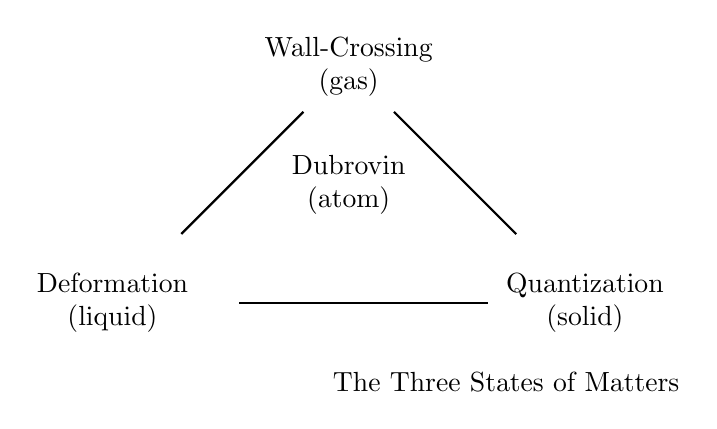
\begin{tikzpicture}[auto, every node/.style={align=center}]
  \node (a) at ( 0,0) {Deformation\\(liquid)};
  \node (b) at ( 6,0) {Quantization\\(solid)};
  \node (c) at ( 3,3) {Wall-Crossing\\(gas)};
  \node (d) at ( 3,1.5) {Dubrovin\\(atom)};
  \draw[-, shorten <= 15pt, shorten >= 3pt, thick] (a)  -- (b);
  \draw[-, shorten <= 15pt, shorten >= 3pt, thick] (a)  -- (c);
  \draw[-, shorten <= 15pt, shorten >= 3pt, thick] (b)  -- (c);
  \node at ( 5,-1) {The Three States of Matters};
\end{tikzpicture}
\end{document}
